\documentclass[11pt]{article}

\usepackage{fontspec}
\usepackage{minted}
\usepackage[scale=1]{ccicons}
\usepackage{metalogo}
\usepackage{xcolor,colortbl}
\usepackage{multicol,multirow,booktabs}
\usepackage{graphicx}
\usepackage{bm}
\usepackage{fontawesome}
\usepackage{exsheets}
\usepackage[paper=a4paper, headheight=110pt,showframe=false,
	layoutvoffset=2em,
	bottom=2cm, top=3.5cm]{geometry}
\usepackage[spanish, es-nodecimaldot]{babel}
\usepackage[babel]{microtype}
\usepackage{hyperref}
\usepackage{amsmath}
\usepackage{mismath}
\usepackage{mathrsfs}
\usepackage{gensymb,amssymb}
\setlength{\parindent}{3em}
\setlength{\parskip}{1em}
\usepackage[shortlabels]{enumitem}
\usepackage{subcaption}
\usepackage{wrapfig}
\usepackage[svgnames]{xcolor} % Gestión de colores
%\usepackage{mathspec}
% \usepackage{unicode-math}


% Fonts can be customized here.
\setmainfont[Ligatures=TeX]{Linux Libertine O}
\setmonofont[Scale=0.90,Ligatures=TeX]{Hack Nerd Font Mono}
\usepackage{hyperref}
\hypersetup{
	colorlinks=true, linktocpage=true, pdfstartpage=3, pdfstartview=FitV,%
	breaklinks=true, pageanchor=true,%
	pdfpagemode=UseNone, %
	plainpages=false, bookmarksnumbered, bookmarksopen=true, bookmarksopenlevel=1,%
	hypertexnames=true, pdfhighlight=/O,%nesting=true,%frenchlinks,%
	urlcolor=Maroon, linkcolor=RoyalBlue, citecolor=Blue, %pagecolor=RoyalBlue,%
	pdftitle={},%
	pdfauthor={\textcopyright\ C. Manuel Carlevaro},%
	pdfsubject={},%
	pdfkeywords={},%
	pdfcreator={XeLaTeX}%
}

%% Operadores
\DeclareMathOperator{\sen}{sen}
\DeclareMathOperator{\senc}{senc}
\DeclareMathOperator{\sign}{sign}
\newcommand{\T}[1]{\underline{\bm{#1}}}
\DeclareMathOperator{\Tr}{Tr}
%\NewDocumentCommand{\evalat}{sO{\big}mm}{%
%\IfBooleanTF{#1}
%{\mleft. #3 \mright|_{#4}}
%{#3#2|_{#4}}%
%}


\title{Cálculo avanzado}
\author{Dpto. de Ingenería Mecánica}
\date{Trabajos prácticos 01 y 02}


\begin{document}
% \maketitle

\begin{center}
\framebox[1.0\textwidth][c]{
\huge{\textsc{Cálculo Avanzado}} 
}
\end{center} 

\begin{center}
\vspace{\baselineskip}
\Large{\textsc{Departamento de Ingenería Mecánica}} \\
\textsc{Facultad Regional La Plata} \\
\textsc{Universidad Tecnológica Nacional}
\end{center}

% \vspace{1em}

\begin{center}
\begin{tabular}{r l}
    \textbf{Trabajos prácticos} & 1 y 2 \\
 \textbf{Temas:} & Series y transformada de Fourier. Transformada de Laplace.\\
 \textbf{Profesor Titular:} & Manuel Carlevaro \\
 \textbf{Jefe de Trabajos Prácticos:} & Diego Amiconi \\
 \textbf{Ayudante de Primera:} & Lucas Basiuk 
\end{tabular}\end{center}

\vspace{1em}

\section{Trabajo práctico 01: Series y transformadas de Fourier.}

\subsection{Series de Fourier}
% Stroud test exercise 7, pg. 266
Dé una expresión analítica de la función cuya representación gráfica se muestra a continuación:
\begin{center}
    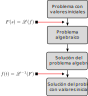
\includegraphics[scale=0.6]{figs/fig-01.pdf}
\end{center}
y compare gráficamente los primeros términos de dicha expresión con la función mostrada.

\subsection{Transformada de Fourier}
Supongamos que tenemos una masa $m$ sujeta a un resorte de constante elástica $k$, a la que se le aplica una fuerza externa $f(t)$ sinusoidal que varía en el tiempo de la siguiente forma:

\begin{equation}
f(t) = A \sen(\omega t)
\end{equation}

Sabiendo que la ecuación diferencial que modea este sistema mecánico vibratorio es:

\begin{equation}
m x''(t) + k x(t) = f(t)
\end{equation}
donde los apóstrofos denotan la derivación respecto del tiempo, hallar la amplitud del movimiento y la diferencia de fase con la función $f(t)$ luego de pasado el régimen transitorio, cuando los valores de las constantes tienen los valores  $m = 5$ y $k = 50$, $A = 1$ y $\omega = 3 \pi / 2$.

Represente gráficamente $x(t)$ y $f(t)$.


\section{Trabajo práctico 02: Transformada de Laplace.}
% Recurso adicional Unit-13-TLaplace.pdf, 13.3, ejemplo 3, pg. 6.
Considere un oscilador de masa $m$ y constante elástica $k$ que se encuentra en un medio viscoso que le provee un amortiguamiento caracterizado por la constante $b$. Si $x(t)$ representa el desplazamiento del oscilador en el instante $t$ desde su posición de equilibrio, el movimiento del oscilador está gobernado por la ecuación diferencial:
\begin{equation}
    m x''(t) + b x'(t) + k x(t) = 0
\end{equation}
cuando no actúa ninguna fuerza externa sobre el oscilador. Aquí $x'(t)$ denota la derivada primera de $x(t)$ respecto del tiempo. Resuelva esta ecuación con los valores particulares $m = 5$, $b = 1$ y $k = 50$, con las condiciones iniciales:

\begin{equation}
\begin{aligned}
    x(0) &= 1 \\
    x'(0) &= -3
\end{aligned}
\end{equation}

Represente gráficamente la solución obtenida.

\end{document}
